%This chapter introduces the SM and the important interactions
%Then top physics is introduced talking about the decay
%tW and tt bar and their crosssections
%What is NLO and LO when are the diagrams similar
%Motivate the difficulties

\chapter{Theoretical basics}

In this chapter the standard model with its elementary particles and interactions is introduced to allow discussing the fundamental kinematics in a particle detector.
Furthermore the analysis in this thesis is motivated and the underlying problems are outlined. For this reason a brief introduction to the theory of particle production and decay is given.


\section{The Standard Model of Particle Physics}
\label{sec:sm}

Originally created in an attempt to unify the electromagnetic, weak ,and strong force under one theory the Standard Model of particle physics represents the status quo in this field summarizing the elementary particles and their interactions.
The model is a gauge quantum field theory and its internal symmetry is the unitary product group $SU(3) \times SU(2) \times U(1)$ in which the interactions are represented by particles named gauge bosons.
Figure \ref{fig:sm} shows the Standard Model particles and their central properties which will be introduced in this chapter starting with the interactions and their mediators followed by a summary of the particles and lastly a section on the top-quark in addition to its properties directly relevant for the research in this thesis.

Although failing to answer open questions like the origin of dark matter or neutrino oscillations, the Standard Model has proven to be a powerful model being very successful in providing experimental predictions for decades.

\begin{figure}
	\centering
	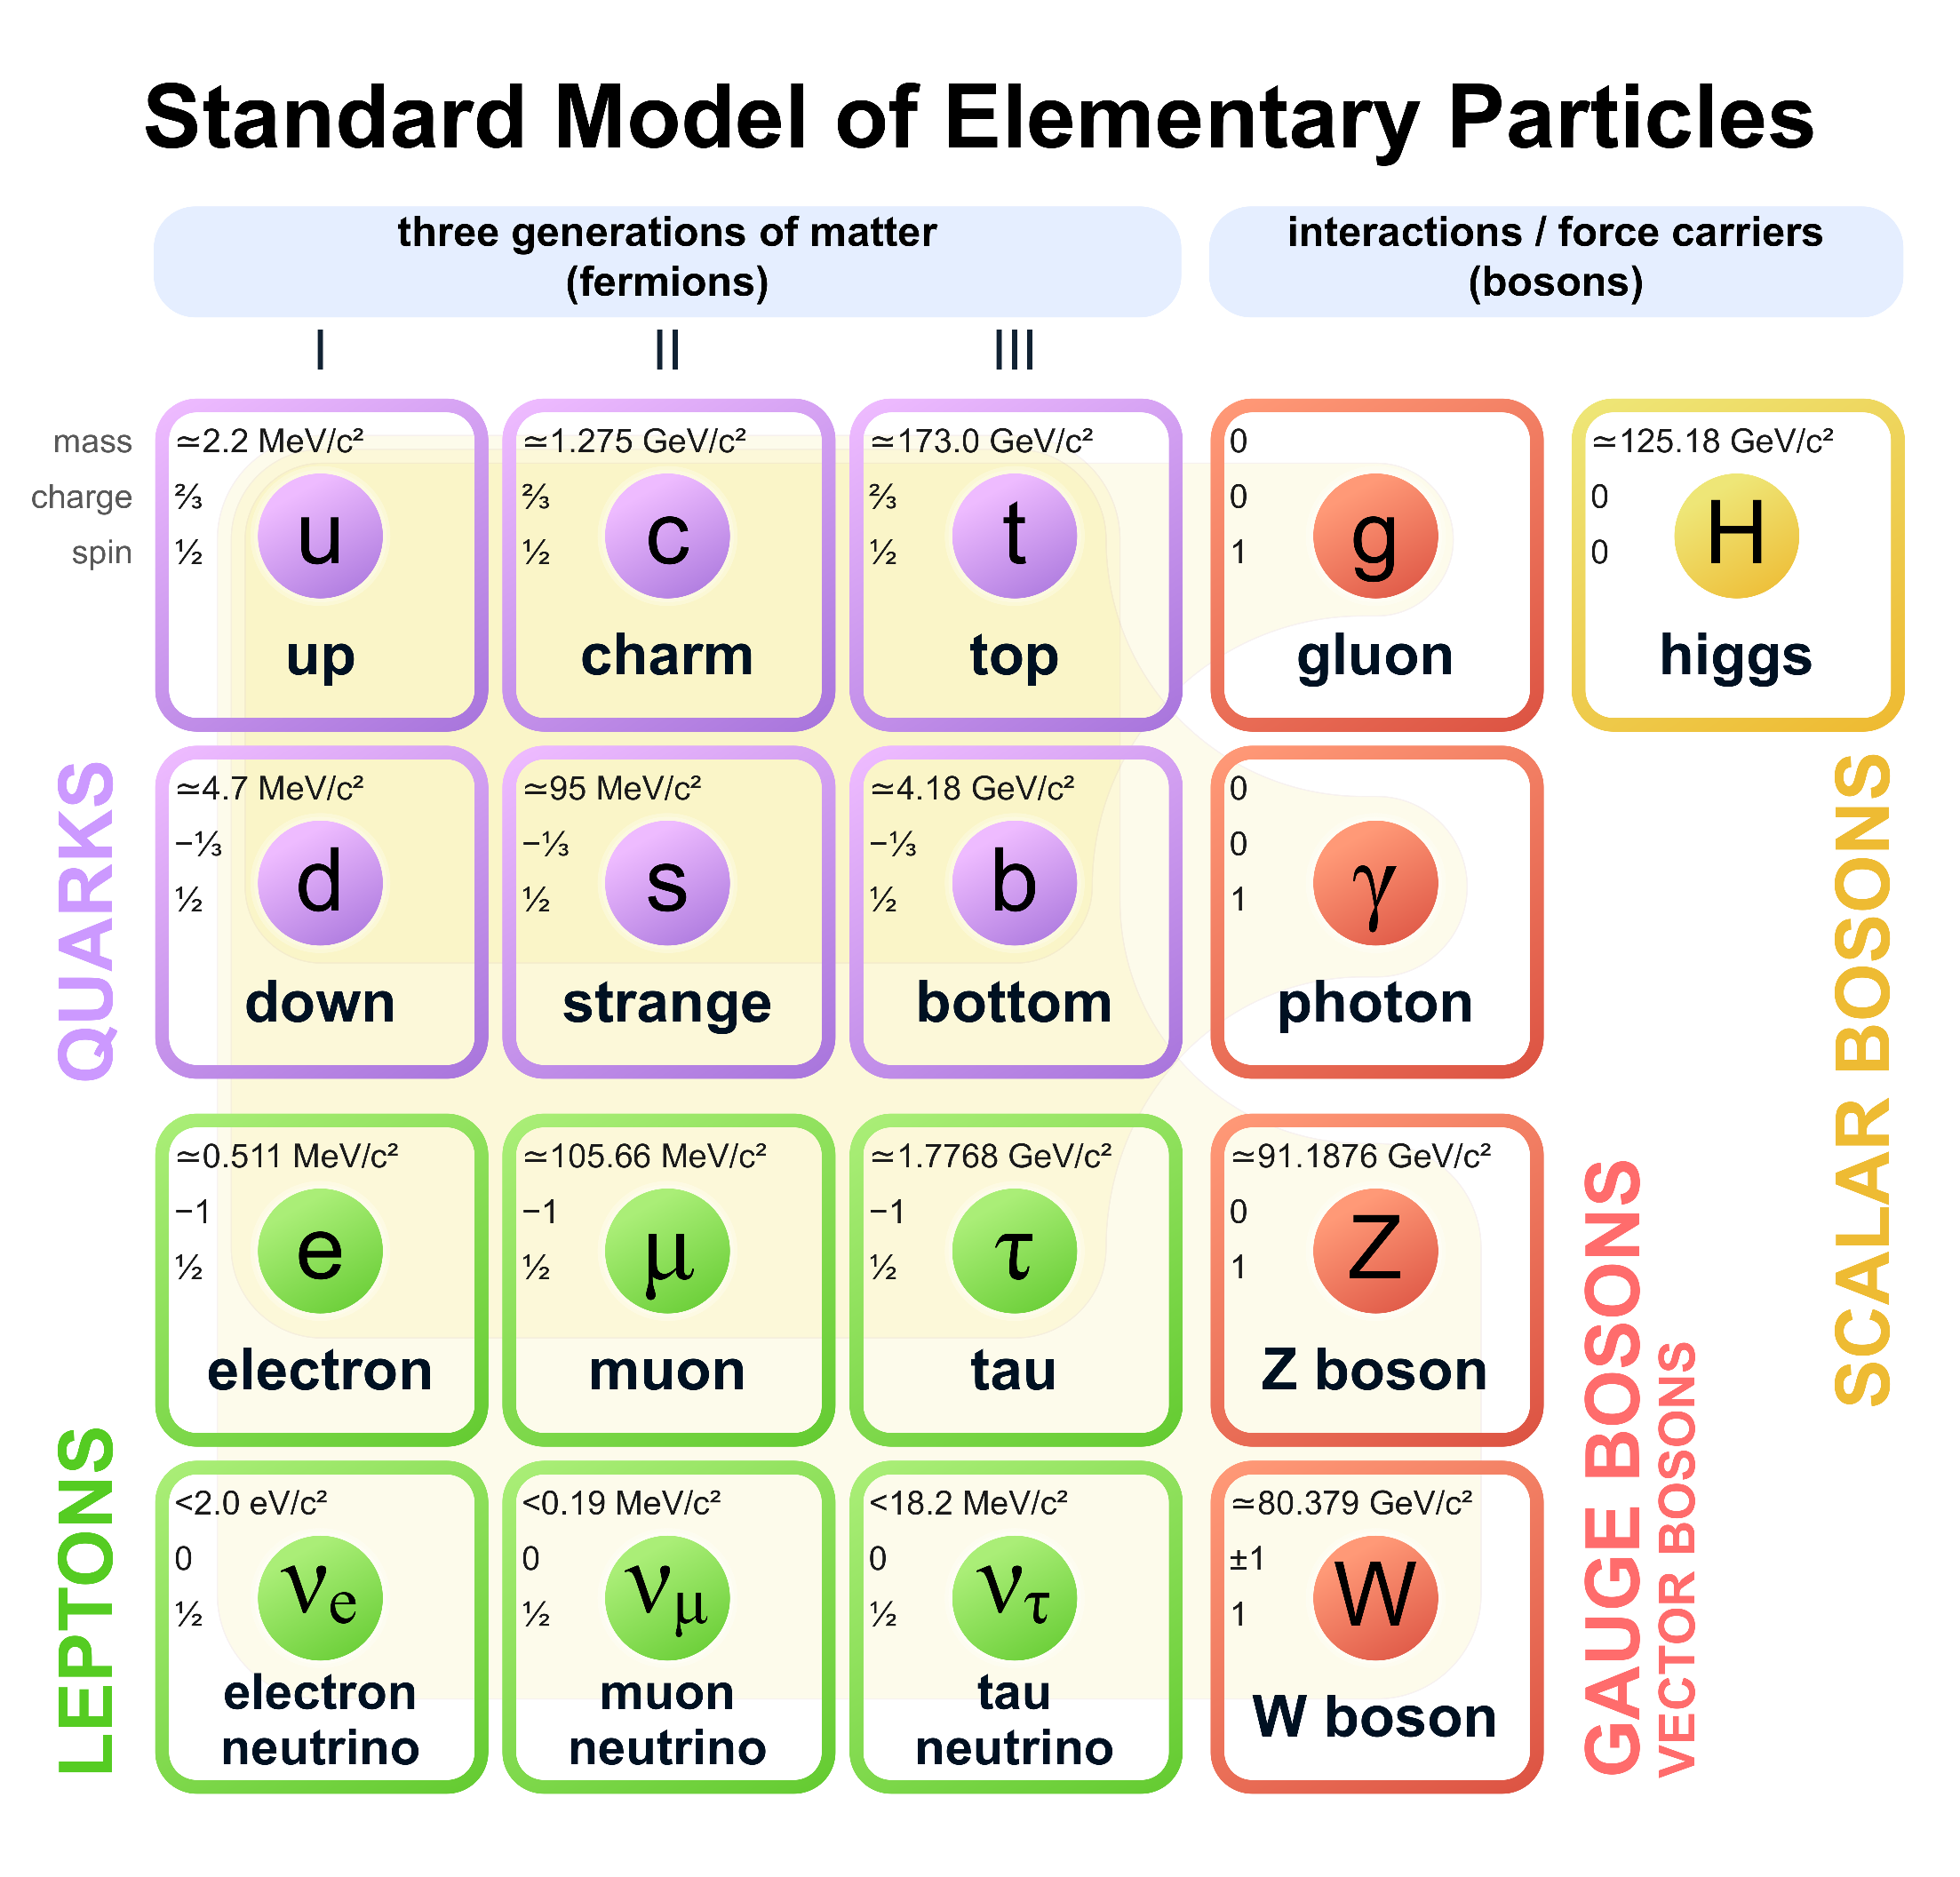
\includegraphics[width=\textwidth]{figures_SM/standard_model.eps}
	\caption[Standard Model particles]{Summary table of the Standard Model particles and their properties. The sketch~\cite{standard_model} was updated to PDG 2018 data~\cite{PDG}}
	\label{fig:sm}
\end{figure}



\subsection{Force carrier particles}

There are three interactions represented in the Standard Model of Particle Physics, the electromagnetic interaction, the weak interaction, and the strong interaction, each represented by a integer-spin particle, called mediator boson. Gravity is usually not included in this model as it is neglectable  at this scale. 

The electromagnetic force is described by the theory of quantum electrodynamics.Its mediator is the photon, a massless particle that couples to the electric charge.
The weak force, most commonly known as the interaction of the $\beta$-decay, couples to the weak charge, an intrinsic property of all fermions, and its mediators are the \PZ- and the two opposite-charged \PW-Bosons.
The electromagnetic and the weak force can be unified as the electroweak interaction forming a $SU(2) \times U(1)$ symmetry.

The strong force is responsible for the binding of quarks in the nucleons. It is mediated by the \num{8} differently flavoured gluons. It only couples to particles with colour charge and is represented by the $SU(3)$ symmetry term in the Standard Model.

As already stated the gravitational force is not included in the standard model as its coupling strength at the scale is only of the order \num{10E-37}. Although it is not a mediator, the Higgs boson was included in the Standard Model after its discovery in 2012.

\subsection{Matter particles}

The non-mediator particles in the model are called \emph{fermions}, which are half-integer spin. They can be broadly classified into three generations of leptons and quarks

The first generation of particles forms the most common form of matter. The electron, the electron-neutrino, and the up- and down-quark, which are the main constituents of the proton and neutron.
In the higher generations the defining quantum numbers stay the same while the mass of the particles increases.
Moreover, there is an antiparticle for each particle with all quantum numbers reversed.

The neutrinos interact only via the weak interaction. There is one neutrino for each lepton-family.
The non-neutrino leptons electron \Pelectron,the muon \Pmu , and the tauon \Ptau have electric charge in addition to their weak charge and therefore also interact via the electromagnetic force.
Furthermore, the six quark flavours are up and down, strange and charm, bottom and top.
The quarks are the only particles interacting with all three forces. They carry not only a weak and an electric charge but also colour charge enabling them to interact with gluons.


\subsection{The CKM matrix}

One aspect of the standard model worth looking at in particular is the CKM matrix which describes the probability of a quark of one flavour generation to be transformed into another quark of suitable charge via the charged weak interaction namely a \PW-boson.
Each parameter $V_{ij}$ represents the probability of a transition between flavour $i$ to flavour $j$. The elements of the matrix predicted with the standard model theory show great agreement to the experimental results.~\cite{pdg}

\begin{align}
\begin{pmatrix}
\Pdown^{\prime} \\
\Pstrange^{\prime} \\
\Pbottom^{\prime}
\end{pmatrix}
&=
\begin{pmatrix}
\Vud & \Vus & \Vub \\
\Vcd & \Vcs & \Vcb \\
\Vtd & \Vts & \Vtb \\
\end{pmatrix}
\cdot
\begin{pmatrix}
\Pdown \\
\Pstrange \\
\Pbottom
\end{pmatrix},\\
%
\begin{pmatrix}
\Pdown^{\prime} \\
\Pstrange^{\prime} \\
\Pbottom^{\prime}
\end{pmatrix}
&=
\begin{pmatrix}
9.97446 & 0.22452 & 0.00365 \\
0.22438 & 0.97359 & 0.04214 \\
0.00896 & 0.04133 & 0.999105 \\
\end{pmatrix}
\cdot
\begin{pmatrix}
\Pdown \\
\Pstrange \\
\Pbottom
\end{pmatrix}.
\end{align}

Important properties not listed in figure xy are the cross-section and the branching fraction.

\subsection{Top quark properties}


The most essential aspects of particle interactions, underlying the events of interest of this work, are the production and decay processes of the top-quark. This section introduces the main properties of the top-quark. Chapter \ref{chp:tW} then expands this explanation by discussing the production and possible decay modes of top-quarks in the Large Hadron Collider (LHC).

The top-quark, being the third generation up-type quark, is special because its mass exceeds the masses of the other quarks by orders of magnitude. Its mass is about \SI{173}{\GeVovercsq} which is higher than the masses of the weak mediators. It almost exclusively decays into a W-boson and a bottom-quark,

\begin{align}
\frac{\Gamma_{\Ptop \rightarrow \PW \Pbottom}}{\Gamma_{\Ptop \rightarrow \PW \Pquark}} = \SI{0.957(34)}{},
\end{align}

and has a lifetime of $\mysim$ \SI{5E-25}{\second} which is smaller than the typical hadronisation time, meaning that the top-quark forms no bound states with other quarks and instead decays.
These essential properties of the heaviest quark lead to some interesting aspects and motivate one to research its properties.
More information on the process involving a top-quark investigated in this is given in chapter~\ref{chp:tW}.
For more information about the standard model see ~\cite{thomson, griffiths}

\section{Feynman diagrams}

%Feynman diagrams
%processes at higher order
%how is ckm related


\section{Kinematics of collider physics}

There are a few kinematic variables and experimental properties worth discussing because they are characteristic for collider experiments which will be briefly introduced in this section.

One of the most important attributes of a collider experiment is its centre-of-mass energy, \Ecms. This denotes the available energy for particle analysis offered by the experiment.
It is defined as:

\begin{align}
\Ecms = \sqrt{ \left( \sum_i E_i \right)^2 - \left( \sum_i p_i \right)^2 }
\end{align}


where $E_i$ and $p_i$ are the energies and momenta of the initial state particles.
In the case of the Large Hadron Collider used for the simulation in this thesis and introduced in chapter \ref{chp:lhc_atlas} two proton beams of equal energy are brought to collision resulting in an energy formula of

\begin{align}
\Ecms = 2 E_{beam}
\end{align}

assuming there are two beams with energies much higher than the particles' masses and therefore one can neglect them in the calculation.

The second property is the luminosity of an experiment which defines how many interactions an experiment can produce. For the colliding gaussian beams underlying the simulations in this work it can be defined as:

\begin{align}
L =f \frac{n_1 n_2}{4 \pi \sigma_x \sigma_y}
\end{align}

where $f$ is the frequency of the beams, $n_i$ is the particle number per bunch and the $\sigma_i$ values stand for the horizontal and vertical beam size respecively.
The integrated luminosity is then used to estimate the total number of interactions for a certain period of measurement:

\begin{align}
\mathcal{L} = \int L(t) dt
\end{align}

Multiplied with a cross-section the corresponding number of interactions to be expected, $N$, can be defined as $N = \sigma \mathcal{L}$.


